\documentclass[a4paper,12pt, oneside]{book}

% \usepackage{fullpage}
\usepackage[italian]{babel}
\usepackage[utf8]{inputenc}
\usepackage{amssymb}
\usepackage{amsthm}
\usepackage{graphics}
\usepackage{amsfonts}
\usepackage{listings}
\usepackage{amsmath}
\usepackage{amstext}
\usepackage{engrec}
\usepackage{rotating}
\usepackage[safe,extra]{tipa}
\usepackage{showkeys}
\usepackage{multirow}
\usepackage{hyperref}
\usepackage{microtype}
\usepackage{enumerate}
\usepackage{braket}
\usepackage{marginnote}
\usepackage{pgfplots}
\usepackage{cancel}
\usepackage{polynom}
\usepackage{booktabs}
\usepackage{enumitem}
\usepackage{framed}
\usepackage{pdfpages}
\usepackage{pgfplots}
\usepackage[cache=false]{minted}

\usepackage{tikz}\usetikzlibrary{er}\tikzset{multi  attribute /.style={attribute ,double  distance =1.5pt}}\tikzset{derived  attribute /.style={attribute ,dashed}}\tikzset{total /.style={double  distance =1.5pt}}\tikzset{every  entity /.style={draw=orange , fill=orange!20}}\tikzset{every  attribute /.style={draw=MediumPurple1, fill=MediumPurple1!20}}\tikzset{every  relationship /.style={draw=Chartreuse2, fill=Chartreuse2!20}}\newcommand{\key}[1]{\underline{#1}}

\usepackage{fancyhdr}
\pagestyle{fancy}
\fancyhead[LE,RO]{\slshape \rightmark}
\fancyhead[LO,RE]{\slshape \leftmark}
\fancyfoot[C]{\thepage}



\title{Programmazione C++}
\author{UniShare\\\\Davide Cozzi\\\href{https://t.me/dlcgold}{@dlcgold}\\\\Gabriele De Rosa\\\href{https://t.me/derogab}{@derogab} \\\\Federica Di Lauro\\\href{https://t.me/f_dila}{@f\textunderscore dila}}
\date{}

\pgfplotsset{compat=1.13}
\begin{document}
\maketitle

\definecolor{shadecolor}{gray}{0.80}
\setlist{leftmargin = 2cm}
\newtheorem{teorema}{Teorema}
\newtheorem{definizione}{Definizione}
\newtheorem{esempio}{Esempio}
\newtheorem{corollario}{Corollario}
\newtheorem{lemma}{Lemma}
\newtheorem{osservazione}{Osservazione}
\newtheorem{nota}{Nota}
\newtheorem{esercizio}{Esercizio}
\tableofcontents
\renewcommand{\chaptermark}[1]{%
  \markboth{\chaptername
    \ \thechapter.\ #1}{}}
\renewcommand{\sectionmark}[1]{\markright{\thesection.\ #1}}
\newcommand{\cpp}{C\texttt{++} {}}
\chapter{Introduzione}
\textbf{Questi appunti sono presi a lezione. Per quanto sia stata fatta una revisione è altamente probabile (praticamente certo) che possano contenere errori, sia di stampa che di vero e proprio contenuto. Per eventuali proposte di correzione effettuare una pull request. Link: } \url{https://github.com/dlcgold/Appunti}.\\
\textbf{Grazie mille e buono studio!}
\chapter{Introduzione a \cpp}
Il \textbf{C++} nasce nel 1983 grazie a Stroustrup durante il suo dottorato
che si occupava di studiare sistemi concorrenti. Conosceva il primo
linguaggio OOP, chiamato \textbf{Simula}, che era comodo per i suoi
scopi ma non riusciva a compilare il codice in maniera
efficiente. Allora decise di passare a \textbf{BCPL} che però non è
tipizzato e non è OOP. Decide quindi di inventarsi un nuovo linguaggio
adeguato ai suoi scopi partendo dal \textbf{C} e unendo i concetti del
\textbf{Simula}, ottenendo il \textbf{C++} nel 1998. Il C++ è
superset del C e quindi è totalmente compatibile con esso. Il C++ è
estremamente versatile, con paradigma procedurale, OOP (\textit{class
  etc$\ldots$}), modulare (\textit{namespace etc$\ldots$}) e generica
(\textit{template etc$\ldots$}). In C++ si ha un ridotto overhead con
una libreria standard semplice e minima, cosa che però costringe a
cercare librerie esterne, spesso non completamente
cross-platform. Nelle ultime versioni del C++ si ha anche
l'introduzione di alcuni costrutti di programmazione funzionale
(\textit{lambda etc$\ldots$}). Tra le ultime novità si annotano:
\textit{multitasking utilities, parallel execution, atomic
  operations, nullptr constant, delegation, initializer\_list,
  automatic type deduction, hash table, smart pointer, tuple,
  espressioni regolari, random number facilities, new mathematical
  functions, type deduction per le classi, easy nested namespace,
  inizializzazioni negli if e switch, concepts, spaceship operator <=>
  etc $\ldots$}. Il codice è al più possibile portabile anche se
ovviamente ci sono limitazioni. Nella scrittura di codice C++ si
preferisce evitare codice ibrido col C anche se è permesso.\\
Il C++ è un linguaggio compilato e i compilatori generano specifici
codici macchina a seconda delle architetture in uso, si ha quindi
portabilità a livello di sorgente (e non a livello di bytecode come
per java, ovvero una volta ``compilato'' in bytecode si può eseguire
l'eseguibile ovunque ci sia una JVM). Essendo portabile a livello di
sorgente (con estensione ``.cpp'' o ``.cc'') ogni volta che si usa una
nuova macchina bisogna ricompilare. In C++ ogni sorgente viene
compilato a parte, producendo un file oggetto (con estensione ``.o'') e infine,
mediante il \textit{linker}, si ha la produzione dell'eseguibile
includendo anche i sorgenti delle librerie esterne indicate. Prima di
produrre il file oggetto si passa per il \textit{preprocessore} che
secondo alcune direttive produce delle \textit{unità di elaborazione}
che vengono poi compilate per produrre i file oggetto. Si ha quindi il
seguente schema:
\begin{center}
  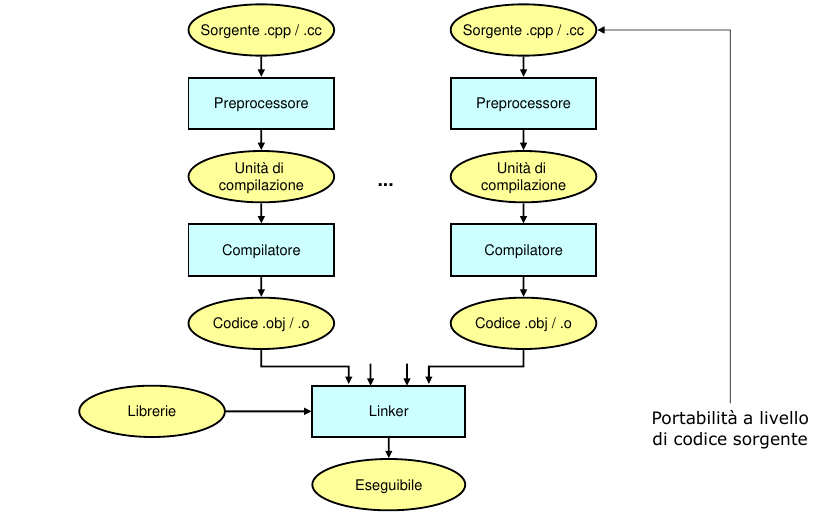
\includegraphics[scale = 0.6]{img/proc.png}
\end{center}
Il preprocessore trasforma un sorgente in un altro interperando delle
direttive nel sorgente indicate col carattere \#. Si hanno 3
gruppi:
\begin{itemize}
  \item le \textit{\#define} che definiscono macro, ovvero sostituzioni di
  stringhe e il compilatore procede con una sorta di find-replace ma
  senza \textit{type-checking} e quindi sarebbero da evitare. Si hanno
  anche le più gravi macro a funzioni. Noi useremo le macro per definire
  TAG. L'opposto di \textit{\#define} è \textit{\#undef}
  \item le direttive \textit{if}, come \textit{\#if \#ifdef/\#ifndef
    \#else/\#elif \#endif} per fare qualcosa in determinate
  situazioni. Comodo nel crossplatforming 8ho linux faccio qualcosa, ho
  windows faccio altro)
  \item le \textit{\#include} per includere altri sorgenti nel sorgente
  in suo (comprese le parti della libreria standard). Si ha sia la forma
  con i doppi apici ("") che con le parentesi angolari (<>) il cui
  comportamento dipende dal compilatore. Normalmente coi doppi apici si
  cerca prima nella cartella di lavoro che nel sistema e viceversa con
  le parentesi angolari
\end{itemize}
\newpage
Nella pratica si ha quanto spiegato nella seguente immagine:
\begin{center}
  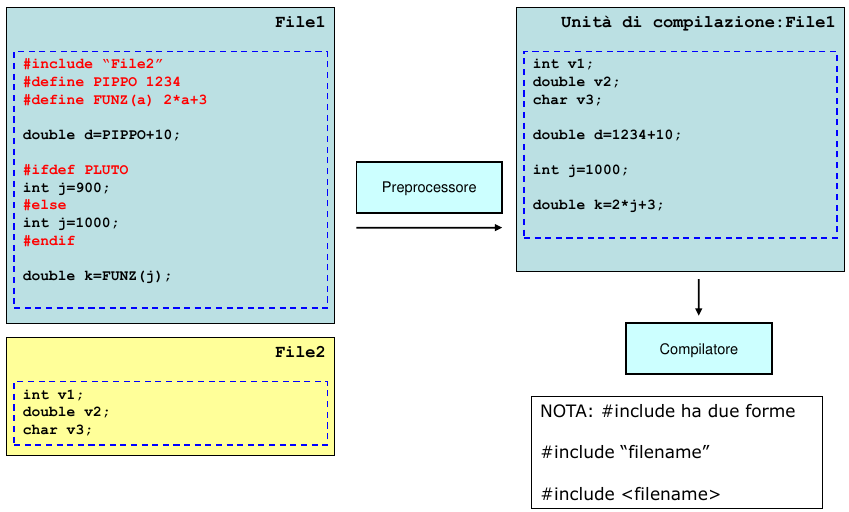
\includegraphics[scale = 0.5]{img/pre.png}
\end{center}
Il compilatore controlla la sintassi (analisi sintattica), il type
checking, le chiamate a funzione (per passarle al linker) e poi genera
il codice il codice di debug. Infine ottimizza il codice e produce il
codice oggetto. Si ha poi il linker che unisce i file oggetto e
elimina codice duplicato o inutilizzato, linkando le varie chiamate a
classi e funzioni. Il linker ha quindi un solo errore:
\textit{``Unresolved External Symbol''}.\textbf{ La compilazione separata
  permette di non dover ricompilare ogni volta tutti i sorgenti}. Infine
il linker aggiunge un codice di startup per l'avvio dell'eseguibile.\\
In C++ si hanno due tipi di sorgenti:
\begin{enumerate}
  \item i file ``.cpp'' che contengono le definizioni di funzioni e
  classi, variabili. Sono compilati separatamente e possono essere visti
  come file di implementazione di una libreria di funzionalità
  \begin{minted}{c++}
    // Dichiarazione funzioni
    // Se non fatto si ha errore
    double f1(double v);
    int f2(int v1, int v2);
    void f3(int v);

    // Funzioni Globali
    double f1(double v)
    {
      ...
    }
    int f2(int v1, int v2)
    {
      ...
      // usa f1()
      ...
      // usa f3()
      ...
    }
    void f3(int v)
    {
      ...
    }
    ...

  \end{minted}
  \item i file ``.h'' \textit{(header file)} che contengono le
  dichiarazioni di funzioni, tipi di dati (classi e simili) e
  variabili. Possono essere visti come file di interfaccia di una
  libreria e sono inclusi dai file ``.cpp'' (e altri file ``.h'') per
  conoscere l’interfaccia di ciò che viene usato. Si permette quindi
  di evitare di ripetere ogni volta le dichiarazioni di qualcosa usato
  in più sorgenti. Si ha quindi il file ``.cpp'' con:
  \begin{minted}{c++}
    #include “file.h”
    // Funzioni Globale
    double f1(double v)
    {
      ...
    }
    int f2(int v1, int v2)
    {
      ...
      // usa f1()
      ...
      // usa f3()
      ...
    }
    void f3(int v)
    {
      ...
    }
    ...

  \end{minted}
  \newpage
  e il file ``.h'' con:
  \begin{minted}{c++}
    // signature (dichiarazioni)
    // di funzioni che voglio far
    // conoscere ad un file .cpp
    double f1(double v);
    int f2(int v1, int v2);
    void f3(int v);
    ...

  \end{minted}
\end{enumerate}
Con la programmazione generica questa divisione viene persa con i file
``.hpp''.\\
\textbf{Per ogni sorgente, escluso il main, bisogna avere un file
  header associato.}\\
Si possono avere inclusioni a vicenda nei vari file header ma questo
può generare problemi avendo più volte l'inclusione di un certo
header. Per ovviare a questo si usano le \textit{guardie}
(\textit{\ifndef, \#define, \#endif}) che sono
direttive del preprocessore che definiscono un TAG solo se non già
definito. Queste sono così usate:
\begin{minted}{c++}
  #ifndef ops_H
  #define ops_H
  #include “common.h”
  // Contenuto di ops.h
  #endif
\end{minted}
\textbf{Si devono usare tag univoci e usare il nome del file con
  l'underscore è comodo (magari in maiuscolo)}.\\
Vediamo ora la differenza tra definizone e dichiarazione. Definire
implica scrivere il codice:
\begin{minted}{c++}
  // definizione funzione
  tipo_ritorno nome(tipo1 var1, tipo2 var2)
  {
    // codice
  }

  // definizione variabile
  tipo1 nome1;
  tipo2 nome2=valore; // inizializzazione
\end{minted}
\newpage
Per dichiarare invece si ha:
\begin{minted}
  // dichairazione funzione
  tipo_ritorno nome(tipo1 var1, tipo2 var2);

  // dichairazione variabile e non alloca memoria
  extern tipo nome; // definizione esterna all’unità  di compilazione corrente

\end{minted}
\textbf{Una dichiarazione è anche una variabile}. Dichiarare più volte
la stessa cosa è rindondante mentre definire più volte è errore.\\
\textbf{Mai includere un ``.cpp'' in un altro}.
\section{Tipi di Dati}
\end{document}